\section{Vedação}
O \cpr possui diversos equipamentos eletrônicos em seu interior que não podem ter contato com água, portanto, para o sistema de vedação realizou-se um estudo dos produtos presentes no mercado que podem realizar a vedação de objetos em água. A seguir apresenta-se um breve descritivo dos principais.

\begin{table}[h]
\centering
\caption{Descrição das principais tipos de adesivos a prova d’água}
\label{table-description-adesivos}
\begin{tabular}{|c|l|}
\hline
\begin{tabular}[c]{@{}c@{}}Cola\\ de\\ resorcinol\end{tabular}                   & \begin{tabular}[c]{@{}l@{}}É um adesivo à prova d'água e forma\\ ligas fortes e duráveis após sua cura,\\ mas a água a remove antes desta cura.\\ O tempo de cura é de 8 a 24 horas,\\ dependendo da umidade e temperatura.\\ A cola de resorcinol precisa de juntas justas,\\ sem folgas,e pressão forte para curar,\\ geralmente, essa pressão é aplicada\\ através de grandes presilhas em C ou presilhas\\ para cola. \cite{ereno2006} A cola de resorcinol tem\\ excelente resistência\\ às temperaturas extremas, produtos\\ químicos e fungos. \cite{ereno2006}\end{tabular} \\ \hline
\begin{tabular}[c]{@{}c@{}}Cola\\ a base\\ de vinil\end{tabular}                 & \begin{tabular}[c]{@{}l@{}}O adesivo a base de vinil têm uma colagem\\ forte à prova d'água em vinil e em\\ muitos plásticos, mas não devem ser usadas\\ em espumas. Normalmente não é necessário\\ usar grampos. A cola de vinil\\ permanece clara e flexível; o tempo de\\ cura é de 10 a 20 min.\end{tabular}                                                                                                                                                                                                                                        \\ \hline
\begin{tabular}[c]{@{}c@{}}Cola\\ a base\\ de epóxi\end{tabular}                 & \begin{tabular}[c]{@{}l@{}}As colas a base de epóxi são de duas\\ partes: uma resina é misturada a\\ um endurecedor, e ela cura por ação química, e\\ não ao ar, como os outros tipos.\\ Ela é a prova d'água, e é muito usada na\\ fabricação de barcos modernos em madeira. Não requer\\ juntas justas, mas preenche as folgas. \\ Precisa apenas de pressão moderada durante a fase de cura.\end{tabular}                                                                                                                                            \\ \hline
\begin{tabular}[c]{@{}c@{}}Cola\\ a base\\ de poliuretano\end{tabular}           & \begin{tabular}[c]{@{}l@{}}As colas a base de poliuretano são aplicadas\\ diretamente do seu tubo, sem precisar de um endurecedor.\\ Ela requer uma junta justa, e\\ a aplicação de pressão durante o tempo de cura. A\\ "DIY Wood Boat" nota que\\ é preciso usar a umidade para curá-la corretamente,\\ então a madeira deve ser\\ levemente umedecida antes da aplicação da\\ cola nas superfícies que\\ ela unirá. Essas colas são a prova d'água. \cite{ereno2006}\end{tabular}                                                                                    \\ \hline
\begin{tabular}[c]{@{}c@{}}Cola\\ a base\\ de ureia e\\ formaldeído\end{tabular} & \begin{tabular}[c]{@{}l@{}}A cola a base de ureia e formaldeído é uma\\ cola de três partes. Um pó deve ser misturado com\\ água para formar uma pasta. Depois,\\ um ácido é adicionado para iniciar o processo\\ de cura. É preciso ter juntas justas e alta pressão\\ para que sua adesão seja apropriada.\\ Ela é resistente à água, mas não completamente\\ a prova d'água.(4)\end{tabular}                                                                                                                                                            \\ \hline
\end{tabular}
\end{table}

Dos adesivos acima descritos, todos possuem uma grande desvantagem, são tóxicos e nem todos são completamente a prova d’água. Com base nisso, procurou-se outro produto no mercado. O Persilox se apresentou como um produto sustentável, não possui cheiro forte e não causa danos à saúde e nem ao meio ambiente, pois sua fórmula inovadora não contém solventes, isocianatos e nem ácidos \cite{adespec2014}. Esse adesivo foi desenvolvido pela Universidade de São Paulo, em sua incubadora, possui um processo de cura é rápido, não retrai, e depois de curado, adquire alto poder de adesão e coesão. Fica completamente elástico, flexível, não trinca, apresentando alta performance em propriedades mecânicas, é resistente a intempéries, radiação $UV$ e pode ser pintado com tintas a base d'água ou outros sistemas \cite{ereno2006}.

\subsection{O Persilox®}
O  Pesilox® é o adesivo a prova d’água, de alta resistênciao, que fará a vedação dos equipamentos elétricos internos.
\par
\begin{figure}[h]
  \centering
  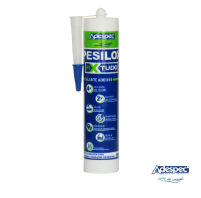
\includegraphics[width=0.4\textwidth]{figures/persilox.png}
  \caption{Adesivo Persilox®}
  \label{fig:persilox}
\end{figure}
\FloatBarrier
\par

O adesivo Persilox® é composto de uma mistura química não é tóxica, como os outros similares da categoria, pois é livre de tolueno, acetado de etila, dentre outros. O Persilox® é um adesivo, impermeabilizante e selante de alta performance que pode ser aplicado em todos os materiais, inclusive em pisos sujeitos a lavagem. O adesivo se solidifica ao entrar em contato com a umidade do ar e, por sua ausência de produtos tóxicos, pode ser aplicado com pano, mão ou pincel. A Tabela \ref{tab:table-compare-persilox} apresenta as características do Persilox®.

\begin{table}[h]
\centering
\caption{Propriedade Química do adesivo à prova d’agua, Persilox®}
\label{tab:table-compare-persilox}
\begin{tabular}{@{}|c|c|@{}}
\toprule
Propriedade                           & PERSILOX                  \\ \midrule
Base química                          & Pesilox                   \\ \midrule
Cor                                   & Preto/Cinza/Branco/Natura \\ \midrule
Mecanismo de Cura                     & Umidade                   \\ \midrule
Densidade                             & 1,35 - 1,40 g/cm\textsuperscript{3}         \\ \midrule
Estabilidade                          & Boa                       \\ \midrule
Temperatura de aplicação              & ambiente                  \\ \midrule
temperatura de formação de película   & 10 minutos                \\ \midrule
Tempo de trabalho                     & 10 minutos                \\ \midrule
Resistência a tração                  & 18 Kgf/cm\textsuperscript{2}                \\ \midrule
Tempo de armazenagem (abaixo de 25ºC) & 12 meses                  \\ \midrule
Resistência a Temperatura             & -40ºC a 120ºC             \\ \midrule
Resistência química                   & muito boa                 \\ \midrule
Trincamento                           & nenhum                    \\ \bottomrule
\end{tabular}
\end{table}

O Persilox® foi utilizado pelo grupo para fazer a vedação da parte elétrica interno do robô. Para testar a eficácia do produto foi feito o teste, descrito no Capítulo \ref{ch:tests-robot} deste relatório.
